\chapter{MÉTODO PROPUESTO}


\section{Conjunto de datos de lesiones de Próstata}

Para el desarrollo de este trabajo, se consideró la cohorte de datos de entrenamiento y desarrollo público \cite{Picai_dataset} contenida en el conglomerado PI-CAI (Prostate Imaging: Cancer AI) \cite{PICAI_BIAS}. Este conjunto de datos es relevante por ser multicentro y multi-equipo. Las secuencias se capturaron en tres centros médicos de los Países Bajos: \textit{Radboud University Medical Center} (RUMC), \textit{Ziekenhuis Groep Twente} (ZGT), \textit{University Medical Center Groningen} (UMCG), en equipos de fabricantes Siemens Healthineers o Philips Medical Systems, con diferentes intensidades de campo (1.5T o 3T). Es longitudinal en el tiempo, con casos de estudio fechados entre 2012 y 2021; homogéneo en sus protocolos, la adquisición se siguió a detalle con lo indicado en el protocolo de imagenología \cite{Engels2020}; e interdisciplinar, en su diseño se contó con un consejo asesor científico internacional compuesto por dieciséis expertos en IA de próstata, radiología y urología.

De la misma manera, estos estudios de resonancia bp-mRI cuentan con las respectivas anotaciones de lesión. Esto implica una segmentación a nivel de vóxel que demarca zonas específicas o regiones dentro de la glándula prostática o en el tejido circundante, así como una posible graduación de la lesión. Estas tareas son realizadas por un profesional capacitado con más de 20 años de experiencia, o un residente bajo la supervisión de un radiólogo. Para lo anterior, se basan en el protocolo de anotación PI-RADS (Prostate Imaging Reporting and Data System), siguiendo las instrucciones de su última versión, la 2.1 \cite{Scott2021}. Por otra parte, es importante mencionar el protocolo ISUP (Histopathological grading of prostate cancer). Aunque ambos protocolos buscan la determinación y estratificación de una lesión prostática y trabajan en el mismo rango [1,5], esto no significa que sean comparables. El protocolo ISUP se destina al reporte únicamente de componentes histológicos, que están en etapas subsecuentes del protocolo de atención; no así las radiológicas que son las establecidas para atención inicial y screening poblacional. Es decir, en este conjunto de datos, los \textit{ground truths} de las lesiones, aunque en un primer momento están determinadas por el radiólogo, se han verificado con el segundo protocolo para confirmar su naturaleza. De acuerdo a lo anterior, se estableció que son casos de estudio positivos aquellos confirmados histológicamente con la denominación ISUP>=2, y negativos aquellos con ISUP <=1 o cuya bm-MRI se haya determinado <=2 y no tengan seguimiento.

En ese sentido, PI-CAI (Prostate Imaging: Cancer AI), cuenta con un total de 1,500 casos de estudio, donde se incluyen además casos del denominado PROSTATEx \cite{Prostatex}, un conjunto precedente de similares características. De todos los casos de estudio, 425 son los que han sido determinados como positivos, con lesión csPCA, pero únicamente 220 son aquellos que están provistos de una marcación asociada, según el estándar ya comentado.


%The MRI sequences were pre-processed following the steps provided by the PI-CAI challenge \cite{saha-picai}. This involved resampling each MRI sequences to a voxel spatial resolution of $0.5 \si{mm} \times 0.5 \si{mm} \times 3.0 \si{mm}$, and then cropping around the center of the scan to obtain a study with 24 slices, each one with size $384 \times 384$. Thereafter, each independent sequence T2, ADC, and DWI were normalized using a min-max normalization to range the values in the interval $[0,1]$.

% In this work, a patch-based approach was followed to create the regions of interest for classification. For this, a volumetric region of interest (vROI) was extracted for each BP-MRI sequence (T2, ADC and DWI) of each case, by centering on the expert annotation with a fixed size of $12 \times 32 \times 32$, where $32\times 32$ are the spatial dimensions in the transverse plane (where $x$ denotes the frontal axis and $y$ the sagittal axis), and $12$ the number of slices, corresponds to the spatial dimension along the vertical axis, denoted by $d$. The respective vROIs are referred to as $\mathbf{X}_{T2}, \mathbf{X}_{ADC}$ and $\mathbf{X}_{DWI}$. For no-csPCa studies, a slice $i_d$ between slices 9 and 15 (included), and a random point at location $(i_x, i_y)$ in the prostate gland on the slice $i_d$ were randomly selected.
% For this, AI-derived delineations of the prostate gland provided by the challenge were used \cite{bosma-ai-delineations}. The vROI was extracted thereafter around the same location $(i_d,i_x, i_y)$ on each sequence $\mathbf{X}_{T2}$, $\mathbf{X}_{ADC}$ and $\mathbf{X}_{DWI}$, see Figure~\ref{fig:vROIS}.

\section{Procesamiento de datos}

En el contexto de este estudio, cada secuencia de los casos de estudio fue sometida a un proceso de preprocesamiento. Para esto, se utilizaron herramientas estandarizadas proporcionadas por el pipeline general descrito en \cite{PICAI_challenge}. Inicialmente, se aplicaron ciertos remuestreos a algunas propiedades de las imágenes; Entre ellos, se modificó el espaciado de los vóxeles a 0.5, 0.5, 3.0 mm y se estableció un tamaño espacial de matriz de 384x384x24. Además, para el nuevo tamaño de imagen, se tuvo en cuenta  centrarse en la glándula prostática. Posteriormente, se alineó cada una de las secuencias contenidas en los casos de estudio con su secuencia principal establecida, en este caso la T2W.  Por otra parte, se tuvo en cuenta la información de metadatos de cada secuencia para alinear las posibles discrepancias en los vóxeles. Finalmente, se verificó que no existieran errores posibles durante el remuestreo para las anotaciones. Esto incluye, por ejemplo, verificar que la conectividad de las lesiones entre slices no haya sido modificada o que el número de lesiones csPCa no discrepe.

Consecuentemente, en el proceso de preparación de los datos para el entrenamiento del modelo, se examinó a nivel de slice cada secuencia de los casos estudio, para identificar aquellos con región csPCA. Al margen de lo anterior, nos valimos de una segmentación apta, exclusiva de la glándula prostática, referida por el algortimo\cite{PICAI_challenge}, entrenado mediante anotaciónes de glándulas prostáticas de \cite{Prostatex_Annotations}. La finalidad del uso de estas segmentaciones es concurrir en áreas prostáticas de interés, mucho más centradas en el órgano, eliminando el ruido de fondo o artefactos.

El procedimiento se sigue así: para los slices donde se correlacionaba una anotación de glándula se establecía un cuadro delimitador de 150 x 150 píxeles, manteniendo el centro glandular constante, proporcionando así un contexto más amplio y garantizando posibles lesiones muy periféricas. 

Por lo demás, estas áreas extraídas se utilizaron como máscaras de recorte y se aplicaron tanto a los slices caso de estudio bpMRI, así como a las anotaciones de lesión. Estas nuevas áreas de los slices de cada secuencia se normalizaron y se combinaron para formar una imagen RGB, es decir, se involucró cada secuencia (T2W, HBV Y ADC) en un canal en la imagen resultante. Estas imágenes RGB son las que contituyen el dataset final de entrenamiento.

En cuanto a las anotaciones de lesión csPCA, indicadas por radiología, se realizó un aumento del 30\% del cuadro que delimita la lesión csPCA marcada por el radiólogo, manteniendo el centro constante, normalizando las coordenadas del cuadro delimitador. Adicionalmente, se llevó a cabo un mapeo de estos cuadros delimitadores csPCA, en el formato [Presencia de lesión, coordenada\_X, Coordenada\_Y, Alto,  Ancho]. Este formato de las anotaciones clarifica de mejor manera las ubicaciones o áreas de interés csPCA, asegurando que se cuente con la información más relevante para la utilización en modelos de localización. 


\section{Red de localización de lesiones significativas de cáncer de Próstata}


% ---> 1 parrafo de resumen muy breve de la arquitectura o los metodologicos que su sigue su red desde la entrada hasta la prediccion ... "En la fgura XX esta el pielene..."

\begin{figure}[h!]
	\centering
	\caption{Pipeline General para la localización de lesiones csPCA}
	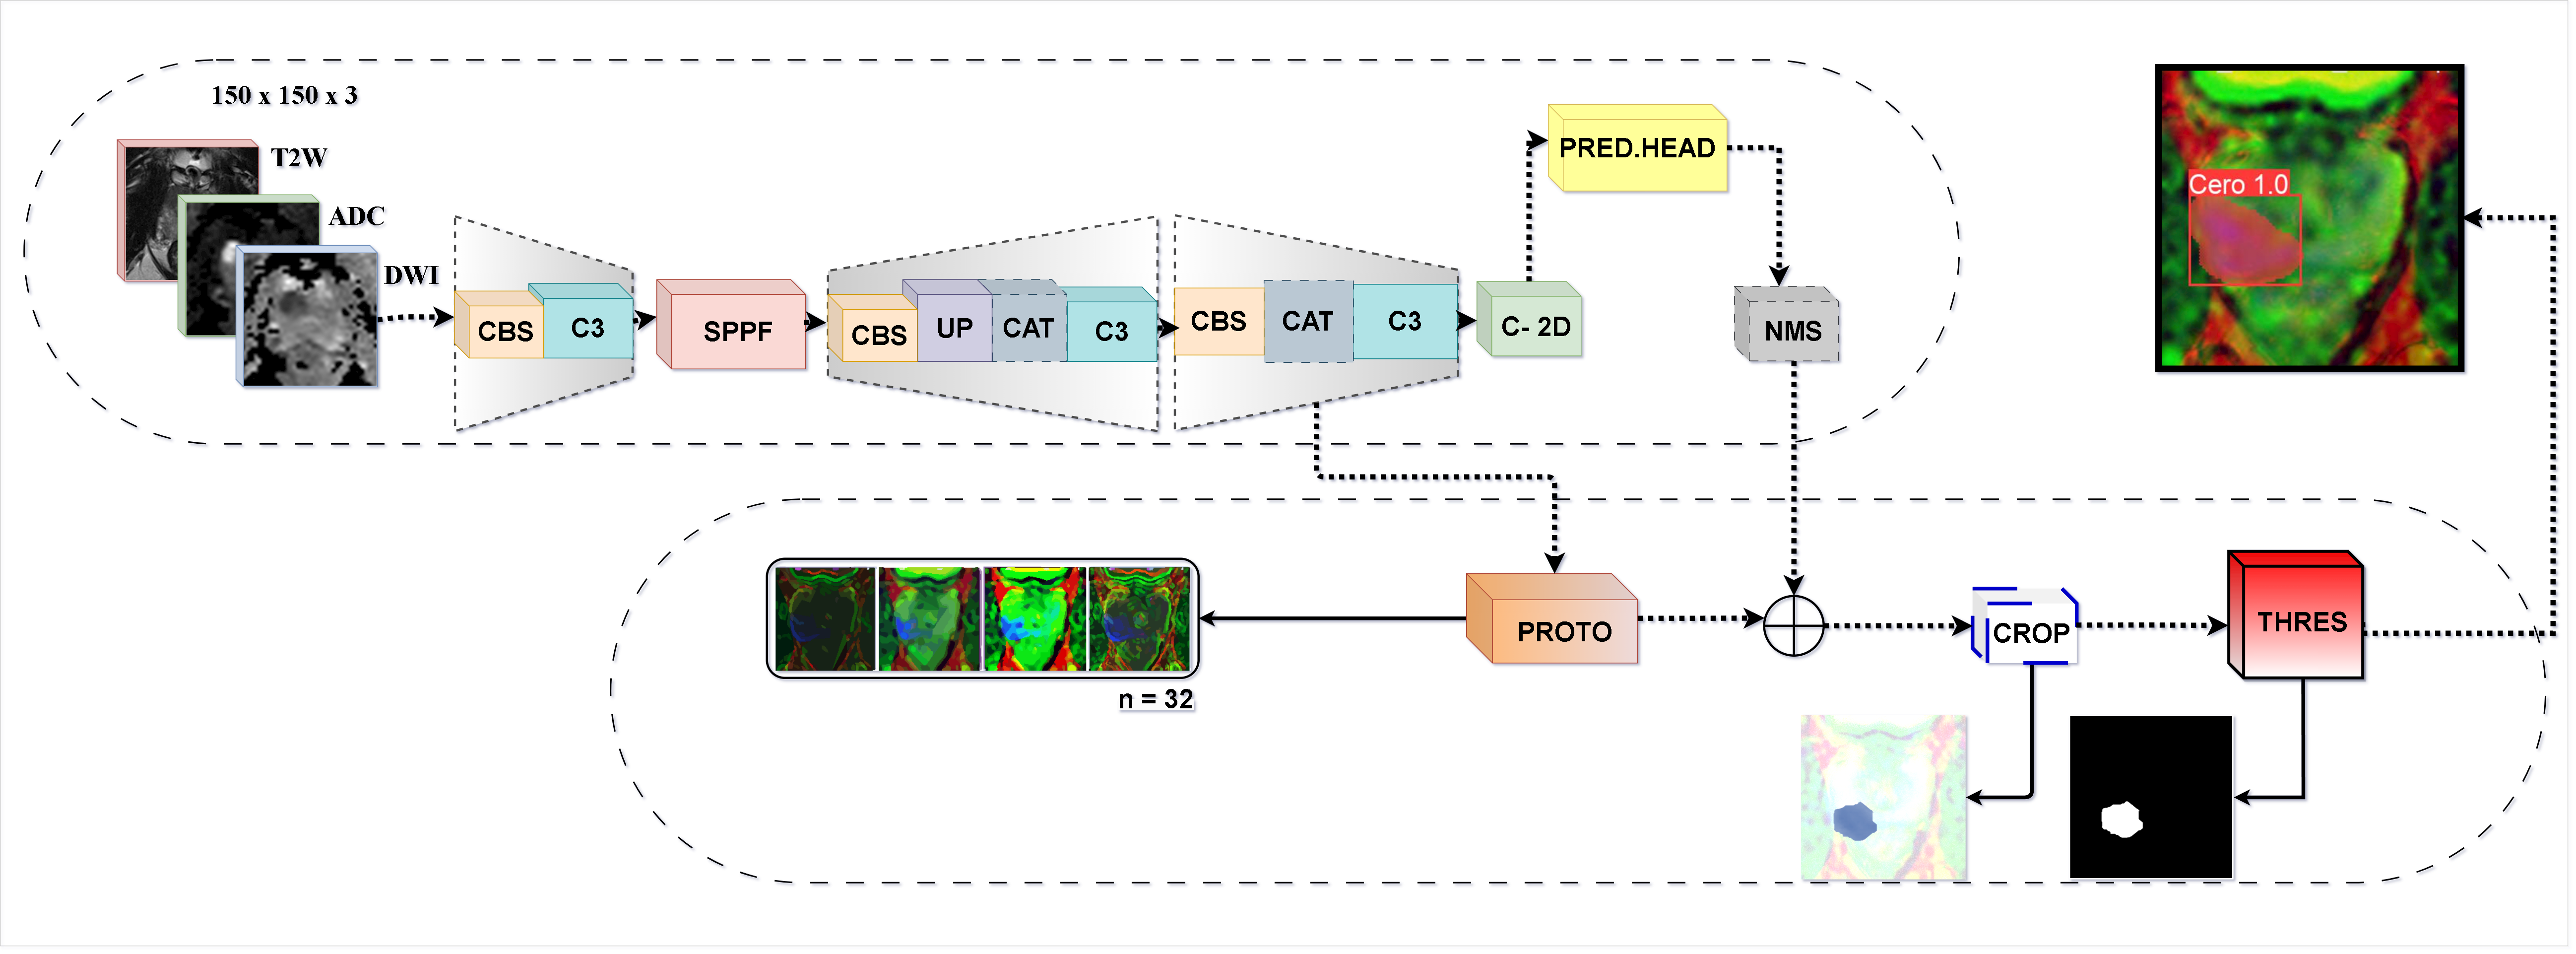
\includegraphics[width=1\textwidth]{imgs/pip_2.png}
	\label{fig:axADC}
\end{figure}

\begin{figure}[h!]
	\noindent \textbf{Nota:} 
	% Figura construida con el uso de datos bp-MRI de próstata de centros médicos de los Países Bajos \footnote{PICAI_BIAS}, y  procesadas con el software ITK-SNAP \footnote{ITKSNAP}.
\end{figure}

% --> Figura del pipeline general [no es tan imporante ser muy detallado con cada componente... porque cada una de ella va a tener su propiea figura... pero si algo ilustrativo por ejempo pequeñas imagenes de activaciones...]

\section{Extracción de características}

% --> Estructura del backbone (incluyendo el upsample)... explicarlo [SPPSSS, y ettc los modulos que contenga..]

% ---> Figura para este bacbone

% ---> Figura con los mapas de saliencia 


\section{Predicción de regiones}

% --> Max supression...

% --> la cabaeza de prediccion [se entender cómo se llegó a los bounding...]

% ---> Figura para esta cabeza de prediccion

% --> La loss ...


\section{Contorno de lesiones para la tarea de localización}

En el procesamiento de imágenes médicas, la identificación precisa de las regiones de interés (ROI) es un componente crítico para el rendimiento óptimo de los modelos de aprendizaje automático. Así pues, se implementó un enfoque alternativo para el tratamiento de las anotaciones de las regiones con lesiones csPCA. En lugar de expandir el cuadro que delimita la lesión del radiólogo un 30\% normalizado, este enfoque implica la identificación de los puntos del perímetro de la lesión csPCA marcada por el radiólogo. Estos puntos se dilatan morfológicamente 5 píxeles, asegurando así que toda la lesión esté incluida. Posteriormente, se normalizan en relación con el tamaño de la máscara de referencia. Este enfoque ofrece una representación detallada de la lesión, lo cual puede potenciar la capacidad del modelo para aprender características relevantes. En términos más detallados, los puntos del perímetro de la lesión se mapean en el formato [Presencia de lesión, coordenada\_X1, Coordenada\_Y1, …, coordenada\_Xn, Coordenada\_Yn]. Este formato de anotaciones proporciona una representación precisa de las áreas de interés csPCA, asegurando que se disponga de la información más relevante para su uso en modelos de localización.

%--> cómo comolas involucra en la red


% ---> Figura sobre como se involucro la segmentacion


%--> Cómo cambió la loss... [se debe entender cómo la red está usando]